\section{Einleitung}
In diesem Kapitel wird die Auftragsgeberfirma Colomba Link vorgestellt. Es wird die Ausgangslage beschrieben und das zu lösende Problem wird eingeführt. Es werden grundlegende Begriffe definiert, die in dieser Thesis von Bedeutung sind.
\gls{abb:HTTP}

The \Gls{latex} typesetting markup language is specially suitable 
for documents that include \gls{maths}. 

\clearpage

\printglossaries
\clearpage

\subsection{Colomba Link}

Die Colomba Link GmbH entwickelt mit Monidas eine IoT-Plattform zur Vernetzung, Verwaltung und Auswertung industrieller Anlagendaten. Sie richtet sich an IoT-Spezialisten sowie Endnutzer und bietet Funktionen von der Einrichtung der Sensoren bis zur automatisierten Überwachung und Alarmierung. Derzeit konfigurieren technische Mitarbeitende die Sensoren kundenspezifisch über eine Weboberfläche (Monidas-Plattform). Komponenten wie Sensoren, Regeln und Benachrichtigungen müssen dabei einzeln erstellt und anschliessend manuell über mehrere Eingabemasken miteinander verknüpft werden. Mit zunehmender Anzahl von Sensoren steigt dadurch der Aufwand für das technische Personal. Aufgrund begrenzter Entwicklungsressourcen verfolgt das Startup das Ziel einer generischen Implementierung, welche Anpassungen und Erweiterungen des Datenmodells sowie den Verwaltungsprozess erleichtert und langfristig zu höherer Kundenzufriedenheit beiträgt. 

\subsection{Konfigurationsprozess}
\label{kap:konf}

Zum Verständnis der in dieser Arbeit beschriebenen Lösung ist es erforderlich, den Aufbau und die Konfiguration der Sensoren in der Monidas-Plattform grundlegend zu kennen. Der folgende Abschnitt erläutert den aktuellen Ablauf der Sensorkonfiguration und stellt relevante Begriffe vor. Dabei beschränkt sich die Darstellung auf jene Aspekte, die für die Problemstellung und die entwickelte Lösung von Bedeutung sind.

Die Konfiguration eines Sensors auf der Monidas-Plattform erfolgt über Eingabemasken. Dabei handelt es sich um Benutzeroberflächen, auf denen Informationen eingegeben und Optionen ausgewählt werden können. Erst wenn alle erforderlichen Konfigurationselemente erstellt wurden, können sie im Monitor zusammengeführt werden. Dieser verknüpft sämtliche Elemente miteinander und ermöglicht dadurch die Überwachung des Sensors.

Im Folgenden werden die einzelnen Konfigurationselemente näher beschrieben:

Actions definieren, wann und unter welchen Bedingungen eine Benachrichtigung versendet wird. Eine Benachrichtigung ist eine Mitteilung, die an vordefinierte Empfängergruppen gesendet wird. Dabei kann festgelegt werden, dass eine Benachrichtigung bei bestimmten Sensorzuständen (Idle, Alert oder Alarm) ausgelöst wird. Zusätzlich wird konfiguriert, ob die Benachrichtigung bei jedem Auftreten des Zustands oder nur einmalig versendet werden soll. Eine Benachrichtigung setzt sich aus zwei zuvor eigenständig erstellten Elementen zusammen, der Group und dem Template. Diese beiden Konfigrationselemente werden über separate Eingabemasken konfiguriert und anschliessend in der Action zu einer Benachrichtigung zusammengeführt.

Die Group legt fest, wer benachrichtigt wird – sie enthält eine Liste von E-Mail-Adressen. Aktuell unterstützt die Plattform nur den Versand per E-Mail.

Das Template bestimmt, was in der Benachrichtigung steht – also Betreff und Nachrichtentext, die in der E-Mail angezeigt werden.

Functions ist für die Logik der Sensordatenauswertung zuständig. Das technische Personal definiert diese Logik direkt im Editor der Monidas-Plattform mithilfe von JavaScript-Code. Dabei handelt es sich um ein einfaches Texteingabefeld ohne Syntaxhervorhebung oder Autovervollständigung. Zusätzlich kann technisches Personal ein JSON-Schema erstellen, in dem Variablen als Properties definiert werden. Innerhalb der programmierten Logik kann anschliessend auf diese Properties über die im Code verfügbare Variable ruleConfig zugegriffen werden. Die Zuweisung der Properties erfolgt entweder direkt innerhalb der Funktion oder zu einem späteren Zeitpunkt über die Benutzeroberfläche im Rahmen der Sensorkonfiguration. Dabei dient das General-Schema als Master-Schema, welches sämtliche definierten Variablen enthält und vom technischen Personal gepflegt wird. Basierend darauf lässt sich zusätzlich ein reduziertes User-Schema definieren. Dieses User-Schema bildet zunächst das General-Schema vollständig ab. Danach können einzelne Properties entfernt werden, indem sie einfach aus dem User-Schema gelöscht werden. Nur die im User-Schema verbliebenen Properties sind später in der Benutzeroberfläche für Endnutzer (z. B. Kunden) sichtbar. Ein konkretes Beispiel für eine solche Funktion zeigt der Temperaturchecker in Abbildung \ref{fig:function}. Diese Funktion analysiert kontinuierlich die eingehenden Sensordaten und entscheidet basierend auf vordefinierten Grenzwerten, ob sich der Sensorzustand im Status ok, alert oder alarm befindet. Wird beispielsweise ein Grenzwert mehrfach überschritten, ändert sich der Zustand des Sensors entsprechend.

\begin{figure}[H]
  \centering
  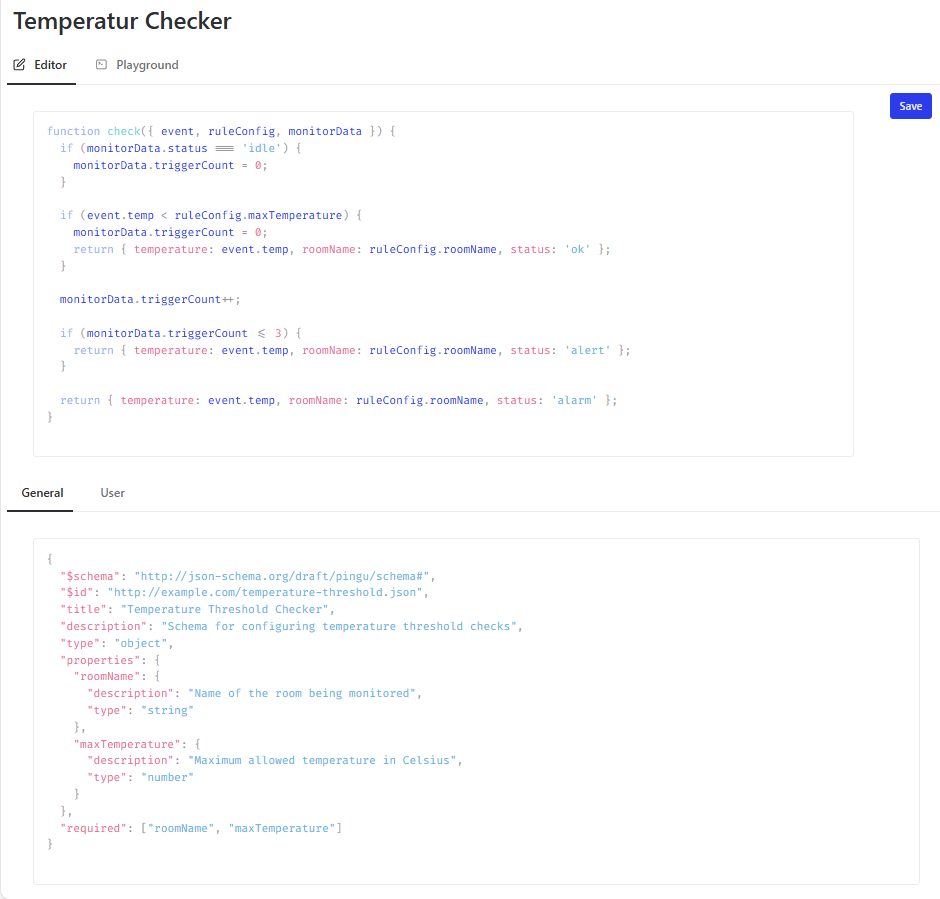
\includegraphics[width=1\linewidth]{function.png}
  \caption{Konfigurationskomponente einer Temperatur Checker Funktion}
  \label{fig:function}
\end{figure}

Nachdem sämtliche Konfigurationselemente definiert wurden, erfolgt ihre Zusammenführung in einem Monitor. Abbildung \ref{fig:monitor} zeigt die Eingabemaske zur Erstellung eines Monitors.

In dieser Eingabemaske lassen sich der Status (Idle oder Alert), der Aktivitätszustand (Active oder Inactive), eine zuvor definierte Function (z.B. der Temperaturchecker), die gewünschten Actions sowie ein Status-Message-Template auswählen. Der Status gibt den initialen Zustand des Sensors an, der sich während des Betriebs ändern kann. Der Aktivitätszustand legt fest, ob der Sensor aktiv überwacht wird oder inaktiv bleibt. Das Status-Message-Template definiert die Nachricht, die bei einem Alarmstatus von der Monidas-Plattform verwendet wird. Im Bereich Rule Config der Eingabemaske befindet sich ein JSON-Editor, über den die im General-Schema der Function definierten Properties gesetzt werden können. Es handelt sich hierbei um ein Textfeld ohne Editorunterstützung. Diese Ansicht ist nur für den technischen Entwickler vorgesehen. Alternativ können die Properties nach der Erstellung des Monitors über eine separate Eingabemaske eingegeben werden, welche das User-Schema verwendet und speziell für Endnutzer vorgesehen ist.

\begin{figure}[H]
  \centering
  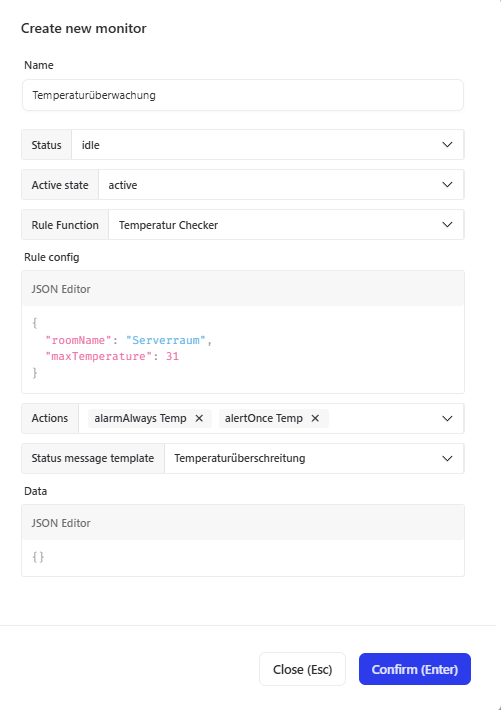
\includegraphics[width=0.7\linewidth]{monitor.png}
  \caption{Eingabemaske zur Erstellung eines Monitors}
  \label{fig:monitor}
\end{figure}

\iffalse
\begin{figure}[H]
  \centering
  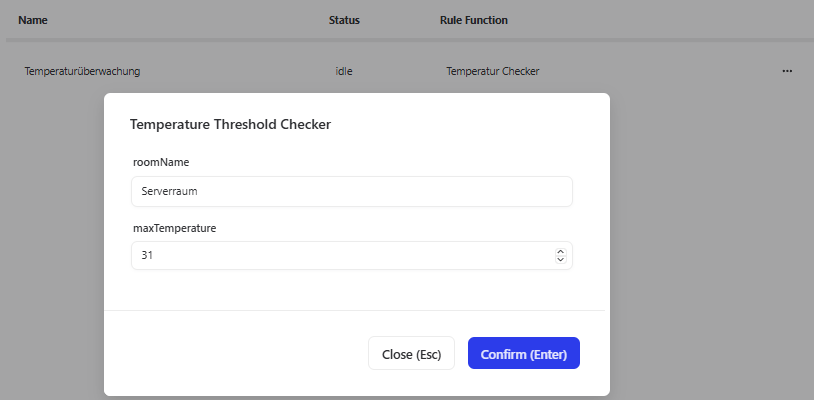
\includegraphics[width=0.7\linewidth]{monitor1.png}
  \caption{Benutzerfreundliche Eingabemaske für Endnutzer}
  \label{fig:monitor1}
\end{figure}
\fi


Nachdem der Monitor vollständig konfiguriert wurde, empfängt und überwacht die Monidas-Plattform kontinuierlich die vom Sensor übermittelten Messwerte. 

Ein Beispiel: Ein Sensor meldet über die API der Plattform einen Temperaturwert von 30 °C. Diese eingehenden Daten werden von der zugeordneten Function verarbeitet. Die Function prüft dabei, ob der gemeldete Temperaturwert innerhalb des zuvor definierten Grenzwerts liegt. Das Ergebnis dieser Auswertung wird dann im Monitor gespeichert. Dort lässt sich jederzeit ablesen, welchen Zustand (z. B. Status „ok“), welche Temperatur, welcher Raum und weitere Informationen die Auswertung ergeben hat. Somit haben Nutzer jederzeit eine Übersicht über den aktuellen Zustand des überwachten Sensors.

Neben dem hier dargestellten Konfigurationsprozess bietet die Monidas-Plattform Möglichkeiten zur Visualisierung und Auswertung der Sensordaten, etwa in Form von Trendanalysen, Diagrammen oder Übersichten aktueller Alarme. Diese Funktionen sind jedoch nicht Gegenstand dieser Arbeit.

\subsection{Problemstellung}
Der in Kapitel \ref{kap:konf} beschriebene Konfigurationsprozess erfordert derzeit, dass verschiedene Konfigurationselemente in einer festgelegten Reihenfolge erstellt werden. Vor der Einrichtung eines Monitors, der die Überwachung eines Sensors ermöglicht, müssen beispielsweise zwingend eine Action sowie eine Function definiert sein. Die Action wiederum setzt voraus, dass zuvor separat eine Group (Empfängergruppe) und ein Template (Inhalt der Benachrichtigung) angelegt wurden. Dies hat zur Folge, dass technisches Personal zahlreiche einzelne Eingabemasken bedienen und miteinander verknüpfen muss, bevor überhaupt ein Sensor überwacht werden kann. Je komplexer das Datenmodell und je höher die Anzahl der Sensoren ist, desto stärker steigt der manuelle, repetitive Aufwand, was die langfristige Wartbarkeit und Skalierbarkeit der Plattform beeinträchtigt.

Neben diesem Aufwand gibt es ein weiteres Problem bei der Konfiguration von Function und Monitor. Für diese Konfigurationskomponenten wird ein einfacher Editor verwendet, der keine unterstützenden Funktionen wie Validierung oder Autovervollständigung bietet. Um solche Funktionen direkt in die Monidas-Plattform zu integrieren, müsste die gesamte Editorlogik eigenständig implementiert und gepflegt werden. Dies verursacht erheblichen Entwicklungs- und Wartungsaufwand. Bei externen Entwicklungsumgebungen wie Visual Studio Code hingegen existieren bereits fertige, modulare Erweiterungen. Diese können ohne grossen Aufwand eingebunden und bei Bedarf flexibel angepasst oder erweitert werden.

Zur Reduktion dieses Aufwands wurde im Vorprojekt IP5 („Entwicklung einer VS-Code Extension zur Verwaltung von IoT-Daten in der Monidas-Plattform“) bereits ein Proof-of-Concept entwickelt, der eine alternative Benutzeroberfläche innerhalb von Visual Studio Code evaluiert. Diese Benutzeroberfläche stellt das Monidas-Datenmodell übersichtlich in einer hierarchischen Baumstruktur (TreeView) dar und ermöglicht eine direkte Bearbeitung der IoT-Daten mittels eines JSON-Editors. Trotz der positiven Ergebnisse des Prototyps offenbarte sich jedoch eine wesentliche Einschränkung: Die Lösung basierte auf einer statischen Integration („Hardcodierung“) des Datenmodells. Dies bedeutete, dass jede Änderung oder Erweiterung manuelle Anpassungen am Quellcode erforderte. Diese starre Implementierung schränkt Flexibilität, Wartbarkeit und Skalierbarkeit deutlich ein und erhöht langfristig den Entwicklungsaufwand.

In dieser Bachelorarbeit wird deshalb eine generische, datenmodellgesteuerte Lösung entwickelt, die diese Einschränkungen beseitigt. Neue Funktionen oder Konfigurationselemente müssen dadurch nicht mehr einzeln auf der Webplattform implementiert werden, sondern können ausschliesslich durch Anpassungen am Datenmodell bereitgestellt werden. Damit werden die Erweiterbarkeit und Wartbarkeit der Monidas-Plattform deutlich verbessert und der Entwicklungsaufwand signifikant reduziert.

\newpage
\subsection{Monidas Code Assist Navigator}
Der Monidas Code Assist Navigator bietet eine alternative Schnittstelle zur Verwaltung und Konfiguration von Daten innerhalb der Entwicklungsumgebung Visual Studio Code. Die Benutzeroberfläche in VS Code besteht aus zwei Hauptkomponenten: einem Explorer und einem Editor.

Abbildung \ref{fig:res} zeigt, wie der Explorer die Daten übersichtlich in einer Baumstruktur darstellt, während der Editor die Bearbeitung der ausgewählten Daten ermöglicht. Die Ansicht des Explorers basiert auf einem Datenmodell, das aus dem Schema der verwendeten Datenbank abgeleitet wird. Der Editor wird durch einen eigenen Language Server unterstützt, der Funktionen wie Code-Analyse, Validierung und Autovervollständigung bereitstellt.

Dank der Nutzung von Visual Studio Code können weitere Entwicklungswerkzeuge, beispielsweise Git, Debugger sowie verschiedene Plugins, direkt verwendet werden.


\begin{figure}[H]
  \centering
  \includegraphics[width=\linewidth]{}
  \caption{}
  \label{fig:res}
\end{figure}

\newpage

\subsection{Forschungsfragen}

Diese Arbeit soll die folgenden Forschungsfragen beantworten:

Welche Architekturentscheidungen sind erforderlich, um den „Code Assist Navigator“ umzusetzen? Welche Auswirkungen hat die Umsetzung des „Code Assist Navigators“ auf die Skalierbarkeit, Erweiterbarkeit und Flexibilität der bestehenden Monidas-Plattform, insbesondere im Hinblick auf das zugrundeliegende Datenmodell? Wo liegen die technischen sowie konzeptionellen Grenzen des „Code Assist Navigators“ bei der Verarbeitung, Darstellung und Navigation komplexer und tiefer Datenmodelle?

\subsection{Abgrenzung}
%Im Rahmen dieser Arbeit werden folgende Themenbereiche nicht behandelt. Die entwickelte Lösung wird nicht in das Produktivsystem von Monidas integriert. Es findet keine Anbindung an die bestehende Webplattform oder das Backend statt. Die Evaluation erfolgt ausschliesslich anhand des Datenmodells, ohne produktive Abläufe zu beeinflussen.

% Nicht berücksichtigt werden ausserdem Funktionen zur gleichzeitigen Nutzung durch mehrere Benutzer, die Benutzerverwaltung, Authentifizierungsprozesse sowie die Rechtevergabe. Auch Themen wie Datensicherheit, Performanceoptimierung, Datenmigration oder die Anbindung externer Systeme sind nicht Bestandteil dieser Arbeit.

Im Rahmen dieser Arbeit werden einige Themenbereiche bewusst ausgeklammert. Die entwickelte Lösung wird nicht in das Produktivsystem von Monidas integriert, und es erfolgt keine Anbindung an die bestehende Plattform. Die Evaluation der Lösung basiert ausschliesslich auf dem Datenmodell.

Ebenfalls nicht berücksichtigt werden Funktionen zur Mehrbenutzernutzung, zur Benutzerverwaltung sowie zu Authentifizierungs- und Autorisierungsprozessen. Themen wie Datensicherheit, Performanceoptimierung oder Datenmigration liegen ebenfalls ausserhalb des Umfangs dieser Bachelorarbeit.

\subsection{Leserführung}
In den folgenden Kapiteln werden die einzelnen Aspekte dieses Projekts genauer behandelt.
 
Kapitel \ref{mon} beschäftigt sich mit der Monidas-Plattform. Dabei wird erläutert, wie die Plattform aufgebaut ist, wie das Domänenmodell definiert wurde und welche Technologien eingesetzt wurden. Berücksichtigt werden Technologien, die für die entwickelte Lösung relevant sind.

Kapitel \ref{schema} behandelt die Anpassungen am Schema. Es wird gezeigt, welche zusätzlichen Schema-Anpassungen notwendig sind, um die entwickelte Lösung umzusetzen. Da das ursprüngliche Domänenmodell der Monidas-Plattform sehr umfangreich ist, wird in diesem Kapitel zudem ein vereinfachtes Domänenmodell eingeführt, welches die entwickelte Lösung verständlich und übersichtlich darstellt. Dieses vereinfachte Modell dient als Grundlage für die Erläuterungen in den Kapiteln \ref{vfs} und \ref{lsp}.

Kapitel \ref{vfs}  behandelt das virtuelle Filesystem. Hier wird erläutert, wie das vereinfachte Domänenmodell aus Kapitel \ref{schema} genutzt wird, um Daten übersichtlich darzustellen und zu bearbeiten.

Kapitel \ref{lsp} befasst sich mit der Editorunterstützung. Es wird gezeigt, wie durch Integration eines Language Server Protocols Validierung, Autovervollständigung und Navigation innerhalb des Editors umgesetzt werden.

Kapitel \ref{sch} fasst abschliessend die Ergebnisse der vorliegenden Arbeit zusammen. Dabei werden die eingangs formulierten Forschungsfragen beantwortet, die entwickelte Lösung kritisch beurteilt sowie mögliche Erweiterungen aufgezeigt.




